\chapter*{HSC Morph Appendix}\label{ch:hsc_morph_appendix}

\section{Data Access}\label{sec_c3:ap:data_access}

GaMPEN's source code is being publicly released along with the publication of this article. Along with the source code, we are also releasing documentation, tutorials, the trained models, the entire catalog of morphological predictions as well as the estimated PDFs for different morphological parameters of the $\sim8$ million galaxies in our sample. 

\vspace{10pt}
Links to the various components of the public data release mentioned above can be accessed at:-
\begin{itemize}
    \item Summary -- \href{http://gampen.ghosharitra.com/}{\url{http://gampen.ghosharitra.com/}}
    \item Summary (Mirror of Above) --\href{http://www.astro.yale.edu/aghosh/gampen.html}{\url{http://www.astro.yale.edu/aghosh/gampen.html}}
    \item Source Code --
    \href{https://github.com/aritraghsh09/GaMPEN}{\url{https://github.com/aritraghsh09/GaMPEN}}
    \item Documentation \& Tutorials -- 
    \href{https://gampen.readthedocs.io/en/latest/}{\url{https://gampen.readthedocs.io/en/latest/}}
\end{itemize}

We caution users to carefully read the Public Data Release Handbook available at \href{https://gampen.readthedocs.io/en/latest/Public_data.html}{\url{https://gampen.readthedocs.io/en/latest/Public_data.html}} to understand various aspects of the data release before using the morphological catalogs produced as a part of this paper. 

Along with the source code and trained models, this public data release also includes the various parameters obtained using the light profile fitting pipeline described in \S \ref{sec_c3:galfitting}.

Since \gampen{} is a living code repository, which we expect to keep changing with time, we have created a ``frozen" version of the code at the time of writing this article. This version is tagged as release \texttt{v0.1.0} in the above-mentioned Github repository and can also be referred to as \citet{gampen_first_release}.

\section{Additional Details About Data}\label{ap:data}

As outlined in \S\ref{sec_c3:data}, we used the \texttt{cleanflags\_any} parameter available as part of HSC PDR2 to exclude objects flagged to have any significant imaging issues by the HSC pipeline. The various triggers which contribute to the above flag, as well as their prevalence among the galaxies which we excluded from the analysis, are shown in Figure \ref{fig_c3:flag_distr}. As can be seen, $\sim80\%$ of the triggers are caused by cosmic ray hits/interpolated pixels. 


In addition, the full SQL queries used to download the low-, mid-, and high-z data are shown in Listings \ref{code:sql_low_z}, \ref{code:sql_mid_z}, and \ref{code:sql_high_z}. Note that after downloading the data using these queries, we further excluded data based on the flags referred to in the previous paragraph, as well as the quality of photometric redshift estimates. For an extended description, please 
refer to \S \ref{sec_c3:data}. As noted in \S \ref{sec_c3:conclusions}, users may additionally choose to use the various \texttt{blendedness} flags available in HSC PDR2 to further exclude merging/blended galaxies. 

\begin{figure}[htb]
    \centering
    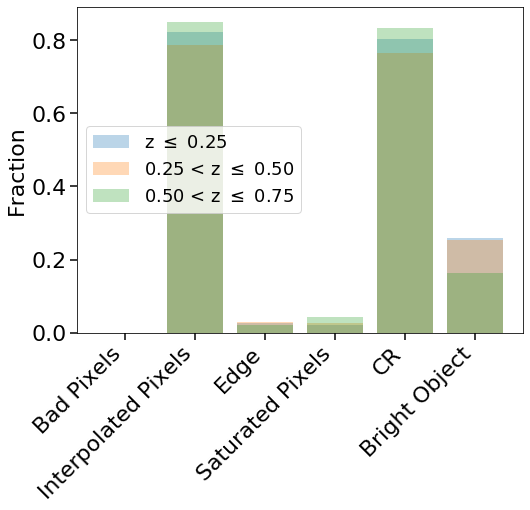
\includegraphics[width = 0.52\textwidth]{flag_distr.png}
    \caption{We exclude $\sim20\%$ of our downloaded galaxies due to different flags being triggered. The distribution of various flags that contribute to galaxies being excluded from our sample is shown in this figure. As can be seen, the large majority of exclusions are due to cosmic-ray hits (and hence, interpolated pixels). }
    \label{fig_c3:flag_distr}
\end{figure}


\begin{lstlisting}[language=SQL, 
    caption={Low-z Sample SQL query}, 
    label={code:sql_low_z}]
SELECT
    object_id
      , ra
      , dec
FROM
    pdr2_wide.smallcat
    LEFT JOIN pdr2_wide.specz USING (object_id)
    LEFT JOIN pdr2_wide.photoz_mizuki USING (object_id)
    WHERE
    ((photoz_best > -1 AND photoz_best <= 0.25) OR (specz_redshift > -1 AND specz_redshift <= 0.25))
    AND (g_kronflux_mag < 23 OR g_cmodel_mag < 23)
    AND g_extendedness_value = 1
;
\end{lstlisting}

\begin{lstlisting}[language=SQL, 
    caption={Mid-z Sample SQL query}, 
    label={code:sql_mid_z}]
SELECT
    object_id
      , ra
      , dec
FROM
    pdr2_wide.smallcat
    LEFT JOIN pdr2_wide.specz USING (object_id)
    LEFT JOIN pdr2_wide.photoz_mizuki USING (object_id)
    WHERE
    ((photoz_best > 0.25 AND photoz_best <= 0.50) OR (specz_redshift > 0.25 AND specz_redshift <= 0.50))
    AND (r_kronflux_mag < 23 OR r_cmodel_mag < 23)
    AND r_extendedness_value = 1
;
\end{lstlisting}


\begin{lstlisting}[language=SQL, 
    caption={High-z Sample SQL query}, 
    label={code:sql_high_z}]
SELECT
    object_id
      , ra
      , dec
      
FROM
    pdr2_wide.smallcat
    LEFT JOIN pdr2_wide.specz USING (object_id)
    LEFT JOIN pdr2_wide.photoz_mizuki USING (object_id)
    WHERE
    ((photoz_best > 0.50 AND photoz_best <= 0.75) OR (specz_redshift > 0.50 AND specz_redshift <= 0.75))
    AND (i_kronflux_mag < 23 OR i_cmodel_mag < 23)
    AND i_extendedness_value = 1
;
\end{lstlisting}


%\section{Additional Details About \gampen{}}\label{ap:gampen}

%To provide readers a visual understanding of how \gampen{}'s different architectural components are organized, Figure \ref{fig_c3:gampen_schematic} shows a schematic diagram outlining the structure of both the STN and CNN in \gampen{}. For complete details on individual layers in \gampen{}, please refer to \citet{gampen_software_paper}.

%\begin{figure*}[htb]
%    \centering
%    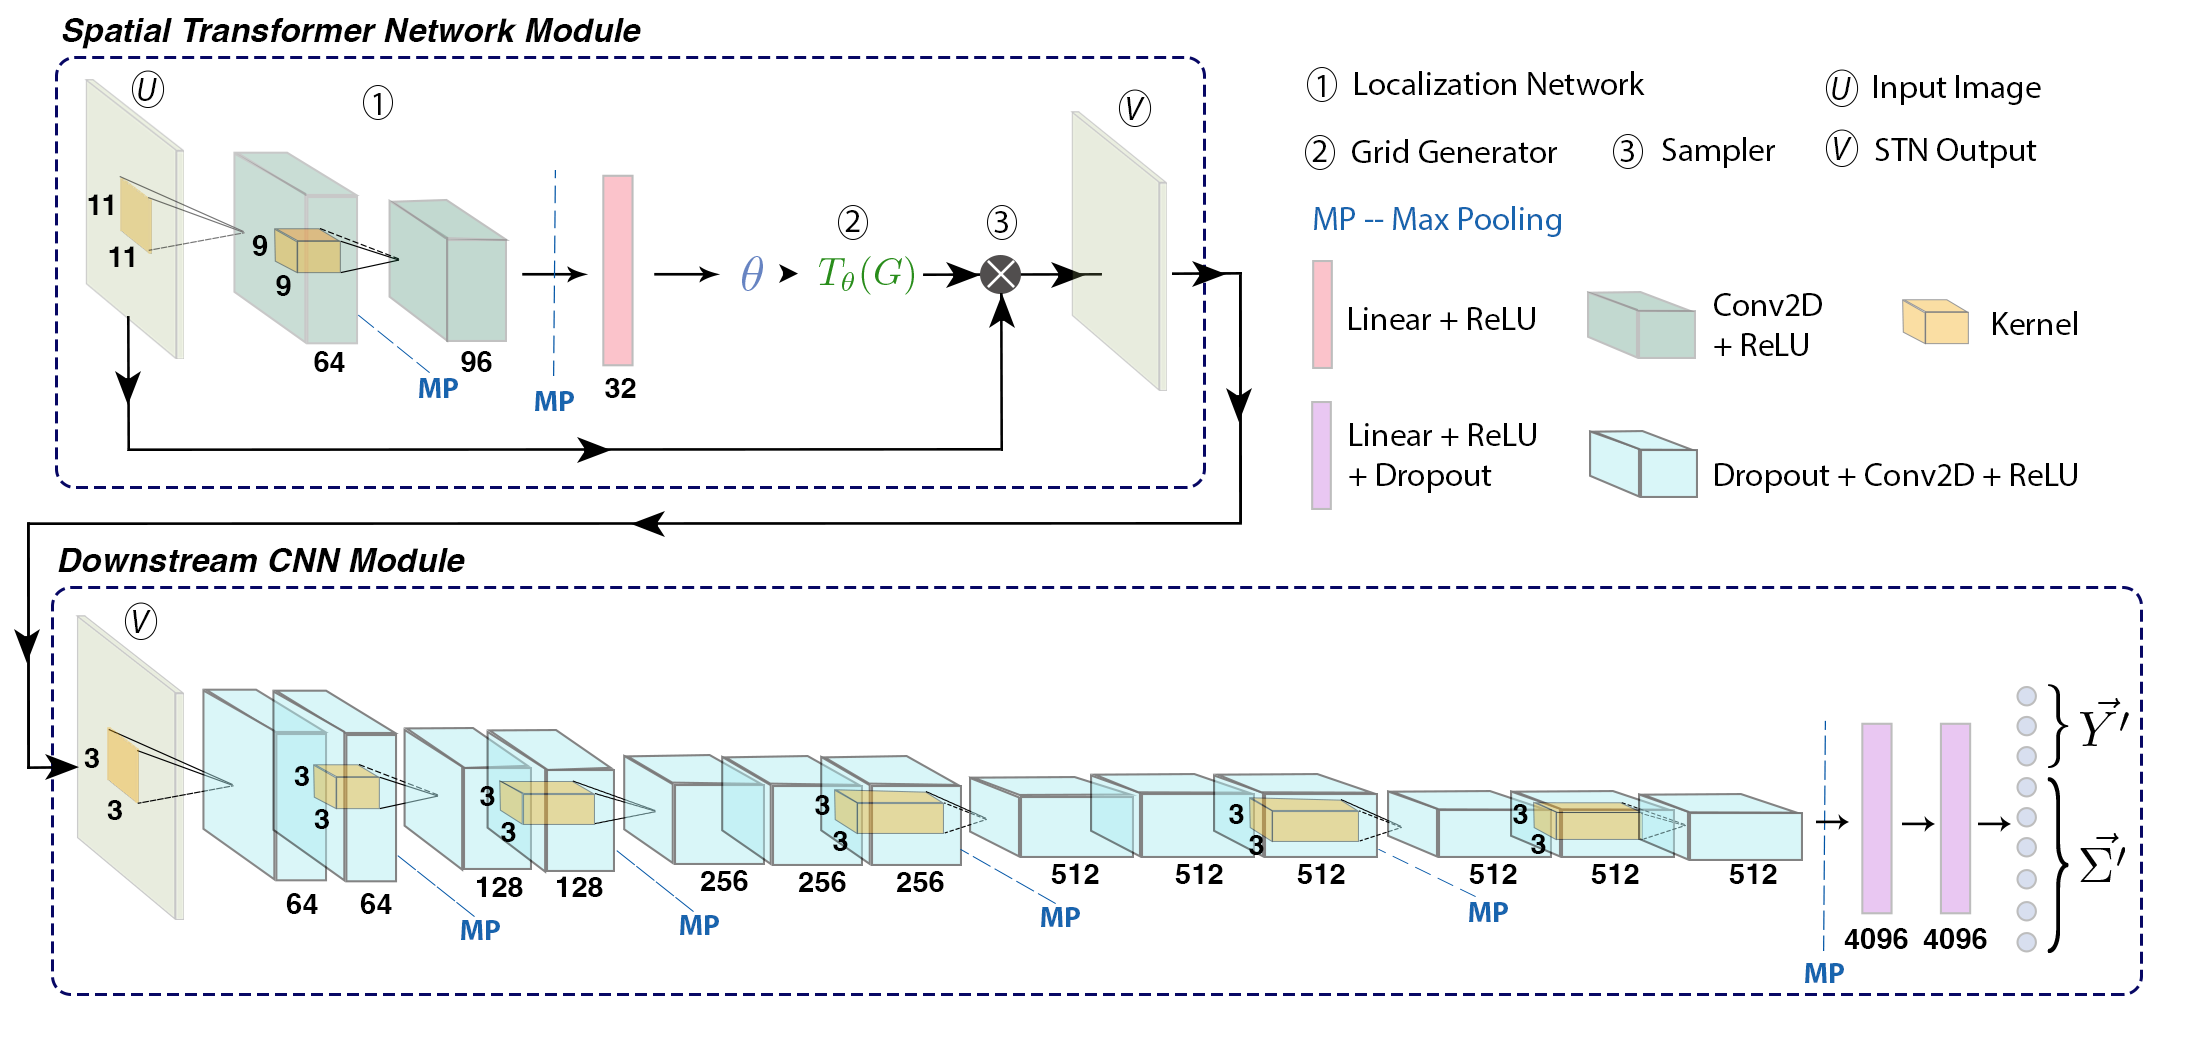
\includegraphics[width
%    =\textwidth]{gampen_schematic.png}
%    \caption{A schematic diagram of the Galaxy Morphology Posterior Estimation Network. \gampen's architecture consists of a downstream CNN module preceded by an upstream STN module. The CNN module empowers \gampen{} to estimate posterior distributions of galaxy morphology parameters. The upstream STN module trains without any extra supervision and learns to apply appropriate cropping transformations to the input image before passing it on to the CNN (for more details about these modules, see \S \ref{sec_c3:gampen}).
%   The numbers below each layer refer to the number of filters/neurons in each layer. The yellow boxes inside the convolutional layers show the kernel and the number beside it refers to the corresponding kernel size. Only one kernel is shown per set of convolutional layers; all other layers in the set have kernels of the same size. Conv2D and ReLU refer to Convolutional Layers and Rectified Linear Units, respectively.}
%    \label{fig_c3:gampen_schematic}
%\end{figure*}

\section{Additional Details About Trained \gampen{} Models}\label{ap:sec_c3:trained_models}

As noted in \S \ref{sec_c3:method}, the training procedure of \gampen{} involves the tuning of various hyper-parameters (e.g., learning rate, batch size, etc.). These hyper-parameters are chosen based on the combination of the values that result in the best performance on the validation data set. The final chosen hyper-parameters for both the simulation trained \gampen{} models, as well as those fine-tuned on real data, are shown in Table \ref{tab_c3:hyper_para}. Please refer to \S \ref{sec_c3:method} for more details on how we train these models.


\begin{table}[htbp]
\centering
\caption{Tuned Values of Various Hyper-parameters  \label{tab_c3:hyper_para}}
\begin{tabular}{c|cccccc}
\hline
\hline
Model& Learning & Momentum & L2 Regula- & Batch & Dropout\\
Name & Rate & & rization ($\lambda$) & Size & Rate\\
\hline
    \hline
    Low-z Sim. Trained & $5\times10^{-7}$ & 0.99 & $10^{-4}$ & 16 & $7\times10^{-4}$\\
    Mid-z Sim. Trained & $5\times10^{-7}$ & 0.99 & $10^{-4}$ & 16 & $7\times10^{-4}$\\
    High-z Sim. Trained & $5\times10^{-7}$ & 0.99 & $10^{-4}$ & 16 & $4\times10^{-4}$\\
    \hline
    Low-z Final & $5\times10^{-8}$ & 0.99 & $10^{-4}$ & 16 & $4\times10^{-4}$\\
    Mid-z Final & $5\times10^{-8}$ & 0.99 & $10^{-4}$ & 16 & $2\times10^{-4}$\\
    High-z Final & $5\times10^{-6}$ & 0.99 & $10^{-4}$ & 16 & $2\times10^{-4}$\\
\hline
\end{tabular}
\end{table}


\section{Identifying Issues with our Light Profile Fitting Pipeline}\label{ap:sec_c3:galfit_failures}

We described in \S \ref{sec_c3:galfitting} a semi-automated pipeline that we used to determine the structural parameters for $\sim60,000$ galaxies using light-profile fitting. After performing this analysis, we visually inspected the fits of a randomly selected sub-sample of $\sim300$ galaxies from each redshift bin, to assess the quality of the fit. 

The process of visually inspecting $\sim 900$ galaxies helped us to identify three failure modes of our fitting pipeline:-

\begin{enumerate}
    \item for some galaxies, GALFIT assigned an extremely small axis ratio to one of the components leading to an unphysical lopsided bulge/disk
    \item for some galaxies, the centroids of the two fitted components were too far away from each other
    \item some galaxies had residuals that were too large
\end{enumerate}

Note that for some galaxies, multiple failure modes were applicable. Examples of each of these failure modes are shown in Figure \ref{fig_c3:galfit_fails}. We use a combination of different cuts on the fitted dataset to get rid of these failure modes -- see \S \ref{sec_c3:galfitting} for an extended discussion. 

\begin{figure*}[htb]
    \centering
    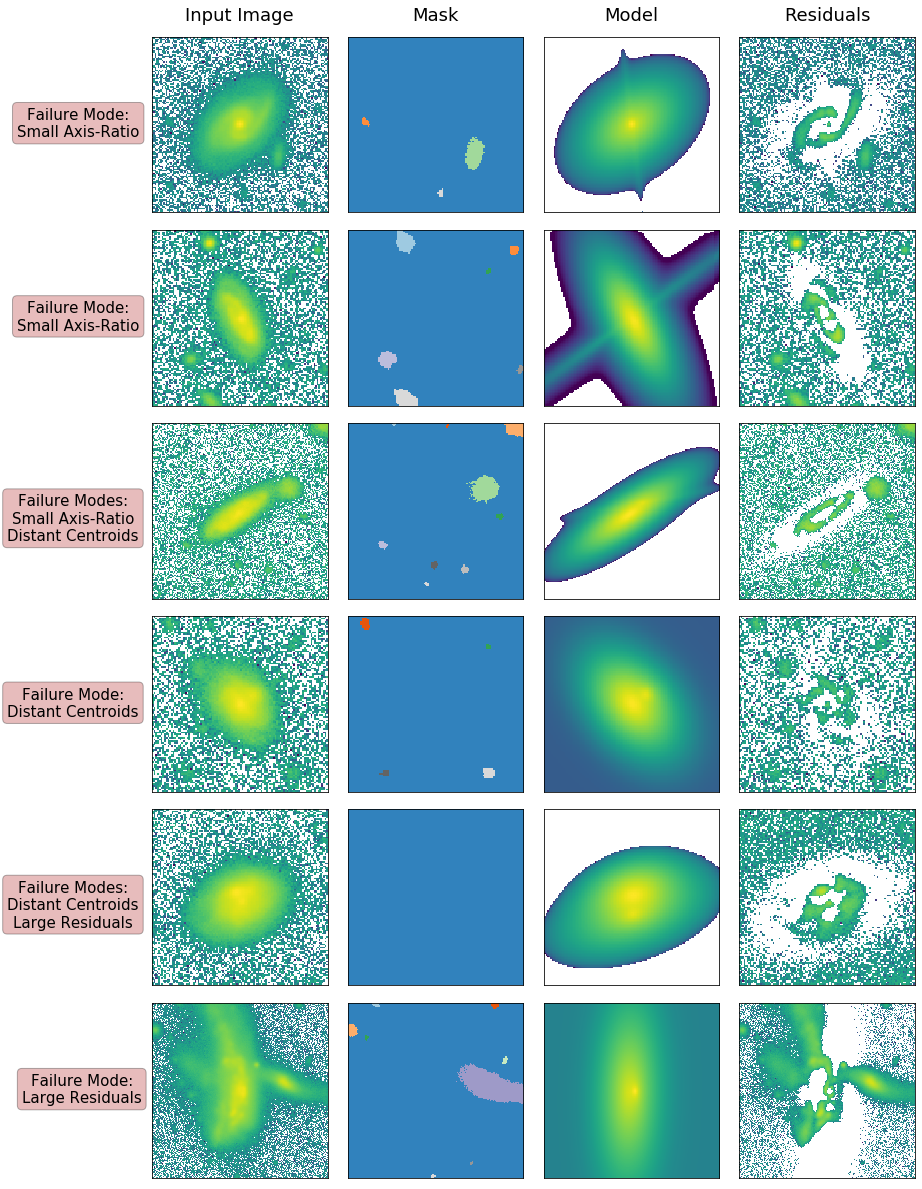
\includegraphics[width = 0.9\textwidth]{galfit_fails.png}
    \caption{The different failure modes of the semi-automated light profile fitting code described in \S \ref{sec_c3:galfitting}. From left to right, we show the input image, the  mask generated by Source Extractor, the model generated by GALFIT, and the residuals.}
    \label{fig_c3:galfit_fails}
\end{figure*}


\section{Additional Two-Dimensional Residual \& Uncertainty Plots} \label{ap:sec_c3:2d_residuals}

Figures \ref{fig_c3:2d_res_mid_z} and \ref{fig_c3:2d_res_high_z} show the distribution of residuals  (difference between \gampen{} and GALFIT predictions) for the mid- and high-z bins. 

Figures \ref{fig_c3:2d_uncer_mid_z} and \ref{fig_c3:2d_uncer_high_z} show the uncertainties predicted by \gampen{} for each parameter plotted against the predicted values for the mid- and high-z bins.

\begin{figure*}[htb]
    \centering
    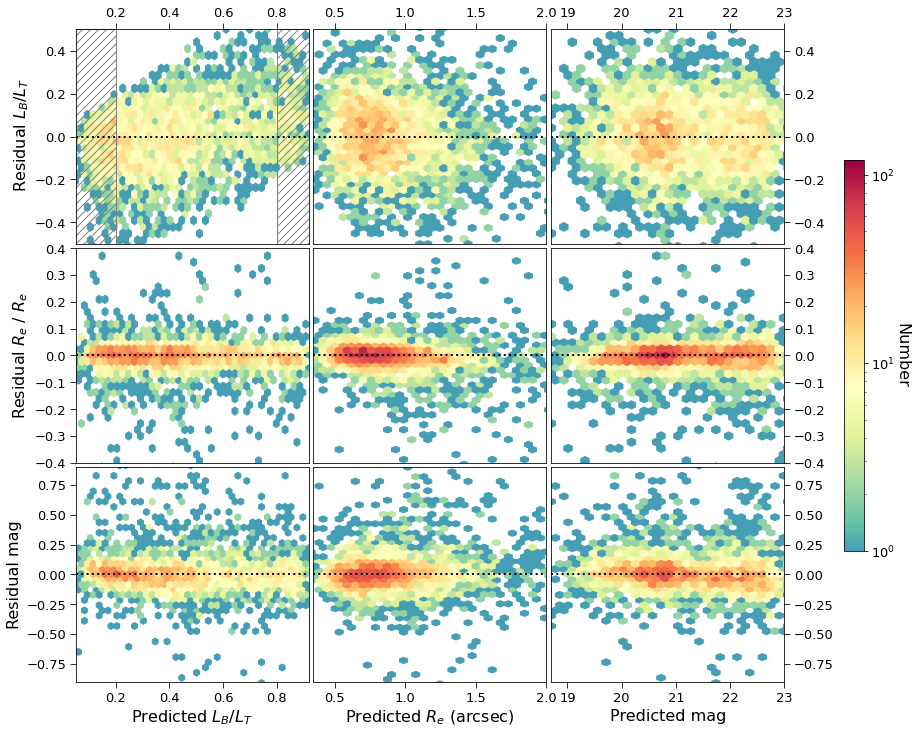
\includegraphics[width = 0.95\textwidth]{2d_res_mid_z.png}
    \caption{Residuals of the output parameters (difference between \gampen{} and GALFIT predictions) plotted against the values predicted by \gampen{} for all galaxies in the mid-z test set. See \S\,\ref{sec_c3:gampen_v_galfit} for details.}
    \label{fig_c3:2d_res_mid_z}
\end{figure*}

\begin{figure*}[htb]
    \centering
    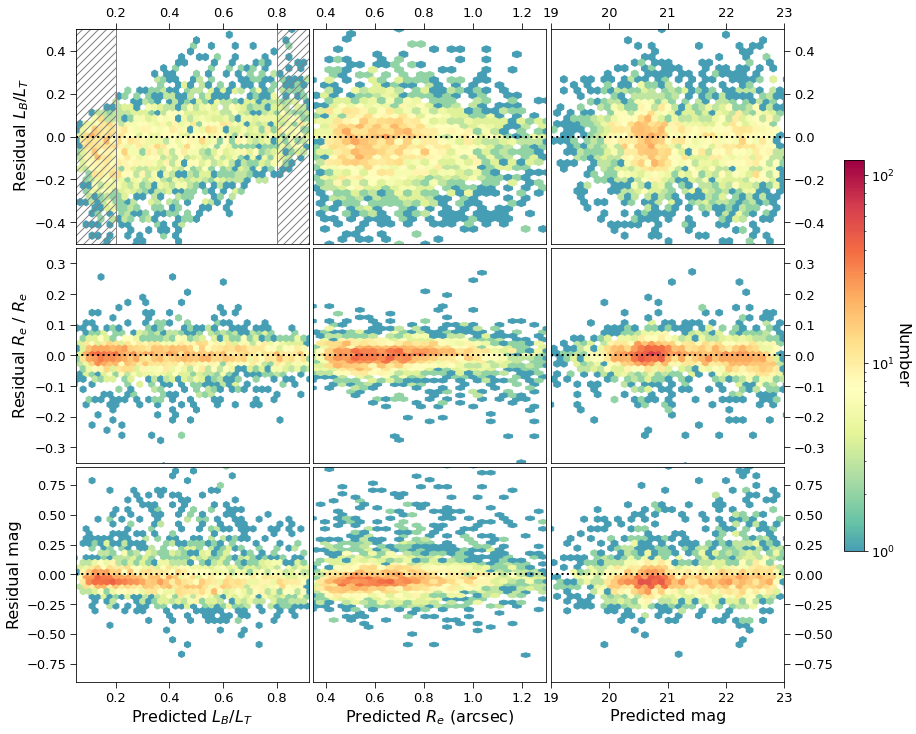
\includegraphics[width = 0.95\textwidth]{2d_res_high_z.png}
    \caption{Residuals of the output parameters (difference between \gampen{} and GALFIT predictions) plotted against the values predicted by \gampen{} for all galaxies in the high-z test set. See \S\,\ref{sec_c3:gampen_v_galfit} for details.}
    \label{fig_c3:2d_res_high_z}
\end{figure*}

\begin{figure*}[htb]
    \centering
    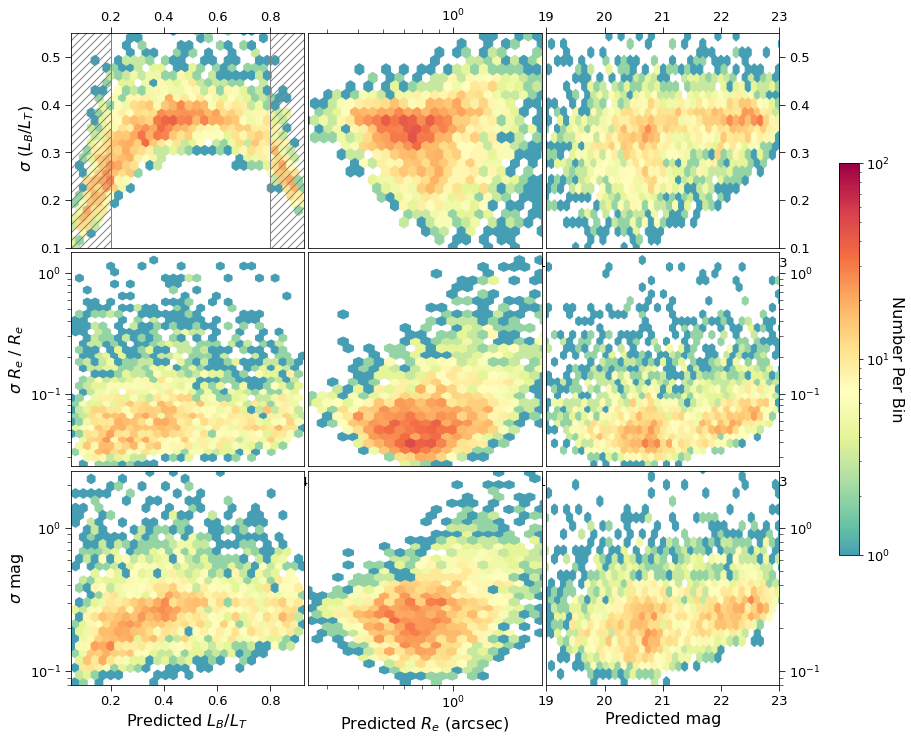
\includegraphics[width = 0.95\textwidth]{2d_uncer_mid_z.png}
    \caption{Uncertainties predicted by \gampen{} for each parameter plotted against the predicted values for the mid-z test set. The $\sigma$ for each parameter is defined as the width of the $68.27\%$ confidence interval. The line-shaded region in the top-left panel shows the region where we recommend transforming quantitative $L_B/L_T$ predictions to qualitative labels. See \S \ref{sec_c3:uncertainties} for details.}
    \label{fig_c3:2d_uncer_mid_z}
\end{figure*}

\begin{figure*}[htb]
    \centering
    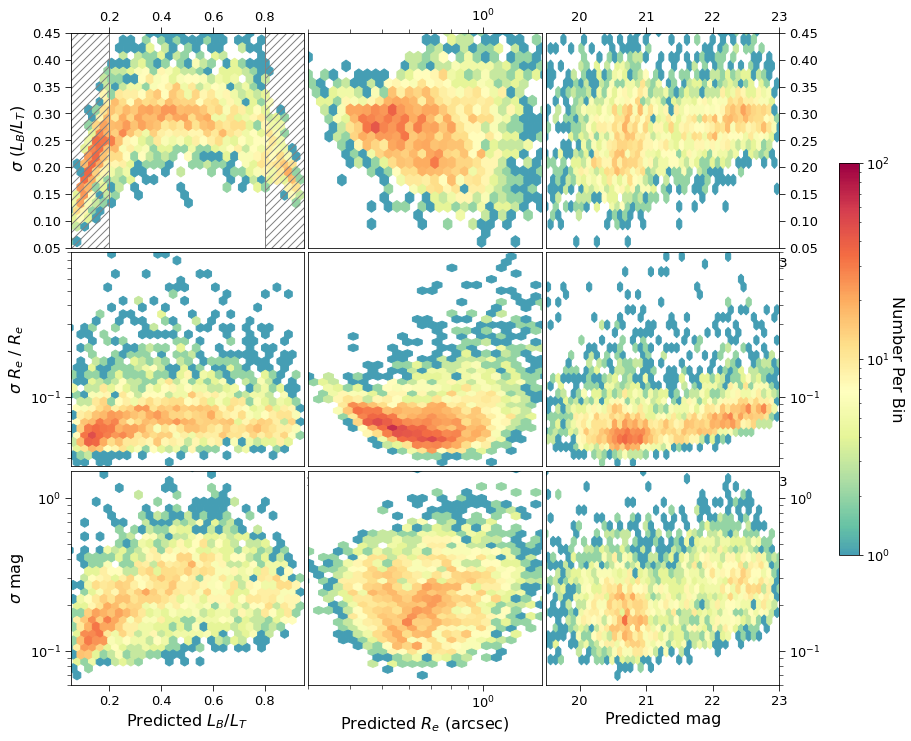
\includegraphics[width = 0.95\textwidth]{2d_uncer_high_z.png}
    \caption{Uncertainties predicted by \gampen{} for each parameter plotted against the predicted values for the high-z test set. The $\sigma$ for each parameter is defined as the width of the $68.27\%$ confidence interval. The line-shaded region in the top-left panel shows the region where we recommend transforming quantitative $L_B/L_T$ predictions to qualitative labels. See \S \ref{sec_c3:uncertainties} for details.}
    \label{fig_c3:2d_uncer_high_z}
\end{figure*}

\section{Comparing \gampen{} and GALFIT's performance on smaller simulated galaxies} \label{ap:sec_c3:gapemn_v_galfit}

As shown in \S \ref{sec_c3:gampen_v_galfit}, GaMPEN and GALFIT systematically disagree more for galaxies with smaller sizes. To ascertain their relative performance, specifically for smaller galaxies, we ran our GALFIT pipeline (described in \S \ref{sec_c3:galfitting}) on $\sim5000$ simulated galaxies from each redshift bin with $R_e \leq 2\arcsec$. These galaxies were chosen randomly from the testing set of \gampen{} -- thus, none of them were used to train \gampen{}. Thereafter, we compared the results of this fitting procedure to the predictions made by \gampen{} on the same galaxies. The residuals obtained for both \gampen{} and GALFIT are shown in Figure \ref{fig_c3:gampen_v_galfit}.

\begin{figure*}[htb]
    \centering
    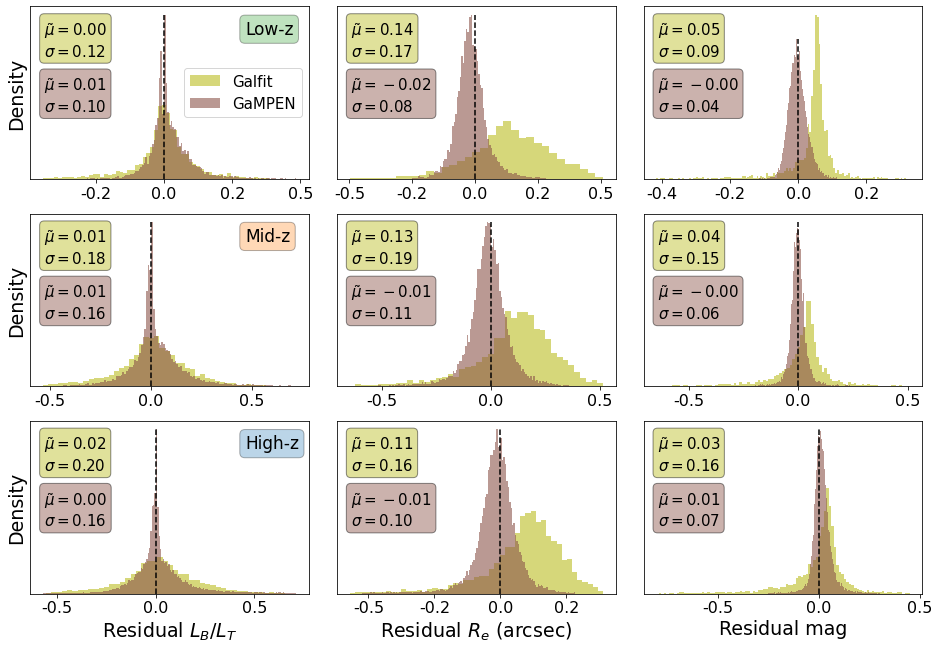
\includegraphics[width = 0.95\textwidth]{gampen_v_galfit.png}
    \caption{Distribution of residuals for $\sim5000$ simulated galaxies in each redshift bin with $R_e \leq 2\arcsec$.  These galaxies were selected randomly from the simulation testing set. The top, middle, and bottom rows show the results for the low-, mid-, and high-z bins respectively. The boxes in the top-left corner of each panel show the median ($\tilde{\mu}$) and standard deviation ($\sigma$) of each residual distribution. The dashed black vertical line marks $x=0$. }
    \label{fig_c3:gampen_v_galfit}
\end{figure*}

The typical error for each of the parameters is given by $\tilde{\mu}\pm\sigma$, where $\tilde{\mu}$ and $\sigma$ are the median and standard deviation of the residual distribution respectively. As shown in Figure \ref{fig_c3:gampen_v_galfit}, \gampen{} outperforms GALFIT for all three parameters across all redshift bins. This provides preliminary evidence that \gampen{}'s predictions on the smaller galaxies referred to in \S \ref{sec_c3:gampen_v_galfit} are more accurate than those obtained using GALFIT.

